%%%%%%%%%%%%%%%%%%%%%%%%%%%%%%%%%%%%%%%%%%%%%%%%%%%%%%%%%%%%%%%%%%%%%%
% How to use writeLaTeX: 
%
% You edit the source code here on the left, and the preview on the
% right shows you the result within a few seconds.
%
% Bookmark this page and share the URL with your co-authors. They can
% edit at the same time!
%
% You can upload figures, bibliographies, custom classes and
% styles using the files menu.
%
%%%%%%%%%%%%%%%%%%%%%%%%%%%%%%%%%%%%%%%%%%%%%%%%%%%%%%%%%%%%%%%%%%%%%%

\documentclass[12pt]{article}

\usepackage{sbc-template}

\usepackage{graphicx,url}

%\usepackage[brazil]{babel}   
\usepackage[utf8]{inputenc}  

\usepackage[portuguese]{babel}

\newtheorem{theorem}{Theorem}[section]
\newtheorem{corollary}{Corollary}[theorem]
\newtheorem{lemma}[theorem]{Lemma}

        
\sloppy

\title{Problema Sanduíche aplicado às classes de grafos cordais e split}

\author{Renan G. da Silva\inst{1}, Natália F. da Silva\inst{1}}


\address{Departamento de Ciência da Computação -- Universidade Federal Rural \\do Rio de Janeiro
  (UFRRJ)\\
  \email{\ renan.gdsilva@gmail.com, natalia-321s@outlook.com}
}

\begin{document} 

\maketitle
     
\begin{resumo} 
  Este trabalho tem como objetivo apresentar e descrever formalmente o problema sanduíche, as classes dos grafos cordais e split e como ambas as classes elas são aplicadas ao problema proposto.
\end{resumo}

\begin{abstract}
This work aims to present and describe formally the Sandwich Problem, the chordal and split graph classes and how either classes are applied in purpose problem.
\end{abstract}

\section{Introdução}

Dados dois grafos $G_1 = (V, E_1)$ e $G_2 = (V, E_2)$, o problema sanduíche busca encontrar uma determinada propriedade $\Pi$ em um grafo $G' = (V, E')$, onde $E_1 \subseteq E' \subseteq E_2$ onde se quer determinar se o grafo $G'$ pertence a uma família ou classe de grafos, como por exemplo se o grafo ele é cordal ou não. O problema sanduíche vem a ser uma generalização do problema de reconhecimento, onde foi introduzido por Golumbic, Kaplan e Shamir \cite{golumbic:95}. Nesse trabalho será explicado com maiores detalhes a respeito o problema sanduíche e a aplicação do problema para a classes dos grafos split e os grafos cordais.

O problema sanduíche possui aplicações nas áreas de mapeamento físico do DNA, raciocínio temporal, sincronização de processos paralelos, árvores filogenéticas, sistemas esparsos de equações lineares \cite{fernanda:2016}.

O trabalho para esta atividade acadêmica tem como objetivo definir formalmente o problema sanduíche, as classes dos grafos cordais e split e o problema sanduíche para essas duas classes. No primeiro capítulo terá, além da descrição do problema brevemente explicado, algumas definições e conceitos básicos que serão discutidos em capítulos posteriores para melhor compreensão, no capítulo 2 serão definidos formalmente as classes dos grafos cordais e split, no capítulo 3 entraremos em detalhes sobre o problema sanduíche e o capítulo 4 com conclusão do trabalho.

%%e o capítulo 4 será apresentado um algoritmo de força bruta para resolver o problema sanduíche para os grafos cordais, ou seja, se dados dois grafos $G_1$ e $G_2$, se existe um grafo $G'$ "ensanduichado" que pertença a classe dos grafos cordais.%%

\subsection{NP-completude}

Alguns problemas aplicados ao problema sanduíche são classificados como $NP$-completos, para os grafos cordais o problema é considerado $NP$-completo, já para os grafos $split$ existe um algoritmo em tempo polinomial. 

Com relação às classes de $NP$-completude, dizemos que um problema é $P$ caso exista algum algoritmo que resolva um determinado problema $\Pi$ em tempo polinomial, ou seja, que o tempo de execução para resolvê-lo é proporcial ao tamanho de sua entrada, algoritmos que classificamos como eficientes possuem complexidade na ordem polinomial, como $O(n^2), O(n log_n), O(n)$. Um problema é considerado $NP$ quando para um determinado problema $\Pi$ existe uma justificativa SIM para o certificado do problema e um algoritmo complexidade polinomial no passo de reconhecimento, caso não exista, não necessariamente esse problema não pertence a classe $NP$. No problema do caminho hamiltoniano, por exemplo, uma justificativa para seu problema é encontrar um ciclo no grafo tal que ao percorrê-lo, não se repita o caminho por uma aresta, um reconhecimento desse problema seria encontrar a resposta NÃO para o seu certificado, por exemplo, caso não haja um ciclo hamiltoniano qualquer no grafo, então deverão ser verificados todos os ciclos no grafo para fazer essa verificação, para o problema do ciclo hamiltoniano, não é conhecido até então um algoritmo eficiente para resolver o problema em tempo polinomial.

Os problemas da classe $NP$-completos são os mais difíceis da classe $NP$ e provavelmente não façam parte da classe dos problemas $P$, essa classe de problemas são um subconjunto dos problemas $NP$, na figura 1 podemos observar um diagrama com as classes dos problemas. Os problemas $NP$-difíceis são problemas tão difíceis quanto os $NP$-completos, com a diferença que a saída do problema $NP$-difícil torna-o um problema de otimização, maiores detalhes a respeito dessa classe podem ser consultados em \cite{JaymeGrafosNovo}.

Existe um problema em aberto envolvendo as classes de algoritmos $P$ e $NP$ onde se quer encontrar a resposta se $P = NP$. Obviamente, ainda não descobriu se existe algum problema da classe $NP$ que seja intratável, ou seja, que não há um algoritmo que o resolva em tempo polinomial. A resposta para esse problema ainda continua em aberto mas que há evidências que direcionam para $P \neq NP$ devido a classe $NP$ possuir muitos problemas, e mesmo assim não foi encontrado um algoritmo em tempo polinomial que os resolva.

\begin{figure}
    \centering
    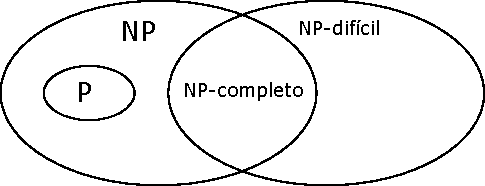
\includegraphics{pictures/diagrama_np.pdf}
    \caption{Diagrama das classes de problemas}
    \label{fig:np_problems}
\end{figure}

\subsection{Definições}

\subsubsection{Esquema de eliminação perfeita}

Um vértice $v$ é considerado simplicial se todos os seus vizinhos $N(v)$ induzirem uma clique maximal do grafo original. Por exemplo, o vértice $a$ do grafo da figura 2 não é simplicial, pois seu vizinho $b$ não induz uma clique maximal.

Um conjunto de vértices ordenados $\phi = v_1, v_2, ..., v_n$ é um esquema de eliminação perfeita se cada vértice $v_i$ removido do conjunto é um vértice simplicial do grafo. Por exemplo, os vértices da figura 1 uma vez ordenados num conjunto $\phi = a, b, c, d$, se para cada vértice removido eles forem simpliciais, então dizemos que existe um esquema de eliminação perfeita.

\subsubsection{Grafos Perfeitos}

Um grafo $G$ é dito perfeito se o número cromático de cada subgrafo induzido for igual ao tamanho da maior clique do subgrafo induzido.

\subsubsection{Grafos Livres}

Um grafo é dito livre de uma determinada propriedade $\Pi$, que podemos usar como exemplo o grafo $K_3$, se não existe em um grafo $G = (V, E)$ um subgrafo com essa propriedade, caso não exista, chamamos esse grafo de $livres$ de triângulos, ou em termos mais práticos, podemos usar a notação $\{K_3\}$-$free$.  

\subsection{Conjunto Independente}

Um conjunto de vértices é dito independente se todos os vértices do conjunto formam componentes desconexas, ou seja, todos os vértices do grafo são isolados, não tendo entre eles nenhuma vizinhança em comum.

\section{Grafos Split e Cordais} \label{sec:firstpage}

\subsection{Grafos Split}

A classe dos grafos $split$ fazem parte do problema de particionamento de grafos, onde se quer particionar o grafo em um conjunto $\phi = v_1, v_2, ..., v_n$ de vértices com algumas propriedades, essas propriedades podem ser por restrições internas ou externas, um exemplo de restrição interna seria uma propriedade dos grafos $split$, onde uma partição deve ser um conjunto independente e uma restrição externa seriam restrições entre subconjuntos \cite{fernanda:2016}. Os grafos split são grafos que fazem parte do problema de particionamento, onde o grafo é particionado em um conjunto independente e uma clique. Brandstädt \cite{brand:96} generalizou a classe dos grafos split e introduziu a classe dos $grafos$-$(k,l)$, onde se quer particionar um grafo $G$ em $k$ conjuntos independentes e $l$ cliques, dizemos então que os grafos $split$ são $grafos$-$(k,l)$, onde $k = l = 1$. Brandstädt em \cite{brand:96}, \cite{brand:98}, \cite{brand:2005} provou que, nos casos onde $k \geq 3$ ou $l \geq 3$ o problema de particionamento pertence a classe dos problemas $NP$-completos e mostrou um algoritmo em tempo polinomial para o reconhecimentos dos $grafos$-$\{(2,1), (1,2), (2,2)\}$.

Os grafos split pertencem à classe dos grafos $(k,l)$, logo, são uma subclasse dos grafos $cordais$ e $perfeitos$. Um grafo é $split$ se e, somente se, for livre de  $C_4, C_5$ e $2K_2$, portanto, essa é uma caracterização dessa classe. Na figura \ref{fig:split_1_1} vemos um exemplo de um grafo split, onde o grafo pode ser particionado em um $K_5$ e um conjunto independente.

\begin{figure}
    \centering
    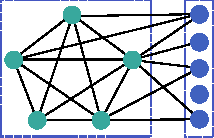
\includegraphics[scale=2]{pictures/(1_1)_graph.pdf}
    \caption{Grafo Split}
    \label{fig:split_1_1}
\end{figure}

\subsection{Reconhecimento de Grafos Split}

Sabemos que um grafo split é um grafo $\{C_4, C_5, 2K_2\}$-$free$, portanto, essas três propriedades classificamos como grafos proíbidos para a classe $split$, um algoritmo para reconhecimento dos grafos $split$ é verificar se o grafo $G$ é livre dessas três propriedades, caso a afirmação seja verdadeira, então o grafo é $split$.

\subsection{Grafos Cordais}

Dado um grafo $G = (V, E)$ é cordal quando o grafo possui todos os seus ciclos com pelo menos tamanho 4 que possuam uma corda em vértices não consecutivos com uma distância ímpar entre os vértices. Grafos cordais também são conhecidos como grafos $triangularizados$. Nas figuras \ref{fig:chordal_1} e \ref{fig:no_chordal} estão alguns exemplos de grafos cordal e não cordal, observamos que o grafo da figura \ref{fig:chordal_1} possui uma corda, que seria o vértice $\overline{ad}$ e o grafo não cordal da figura \ref{fig:no_chordal} não possui as arestas $\overline{ac}$ e $\overline{bd}$ no ciclo induzido $a, b, c, d, a$.

\begin{figure}
    \centering
    
\includegraphics[scale=0.4]{pictures/path55.png}
    \caption{Grafo cordal}
    \label{fig:chordal_1}
\end{figure}

\begin{figure}
    \centering
    
\includegraphics[scale=0.4]{pictures/non_chordal_1.png}
    \caption{Grafo não cordal}
    \label{fig:no_chordal}
\end{figure}

Os grafos cordais são uma subclasse dos grafos perfeitos. Um grafo é dito perfeito quando $\chi(G) = \omega(G)$.

Assim como os $grafos$-$(k,l)$, os grafos cordais também podem ser chamados de $(k,l)$-$cordais$ com a mesma propriedade do problema de particionamento, onde se quer particionar um grafo em $k$ conjuntos independentes e $l$ cliques. 


Há também a definição de grafo $cordal$-$(k,l)$, onde o grafo possui a mesma propriedade do problema de particionamento proposto por Brandstadt, de se particionar o grafo em $k$ conjuntos independentes e $l$ cliques, ou seja, é um $grafo$-$(k,l)$ e ser um grafo $cordal$.

A propriedade ser cordal é uma propriedade hereditária, portanto, qualquer subgrafo induzido de um grafo $cordal$ também será um grafo $cordal$.

\subsubsection{Reconhecimento de Grafos Cordais}

O reconhecimento dos grafos cordais pode ser feito através do algoritmo de busca lexicográfica ($LEX$-$BFS$). O $LEX$-$BFS$ é um algoritmo que se assemelha a busca em largura, porém com critérios de ordenação para exploração dos vértices de um grafo, maiores detalhes a respeito desse algoritmo podem ser conferidos no livro do Szwarcfiter \cite{JaymeGrafosNovo}.

\begin{lemma}
Seja $G = (V, E)$ um grafo cordal aplicado ao algoritmo de busca em largura lexicográfica. Então a sequência S de vértices $v$ ordenados decrescentemente segundo $largura(v)$ é um esquema de eliminação perfeita
\end{lemma}


O algoritmo de busca lexicográfica ($lex-BFS$) ordena todos os vértices do grafo em ordem descrecente, os grafos cordais possuem esquema de eliminação perfeita, portanto, executando o algoritmo $lex-BFS$ sobre um grafo cordal $G$, obtemos os vértices $\phi = v_1, v_2, ..., v_n$ em ordem descrescente, após obter a lista de vértices ordenada, deverá ser verificado se os vértices induzem uma clique, ou seja, se o vértice $v_i$ é simplicial, caso a afirmação seja verdadeira, então os vértices do conjunto retornado $\phi$ é um esquema de eliminação perfeita. Esse algoritmo de reconhecimento de grafos cordais possui a complexidade $O(nm)$.


\section{Problemas Sanduíche}

O problema sanduíche é uma generelização do problema de reconhecimento de classes de grafos, onde se quer determinar se, dados dois grafos $G_1$ e $G_2$, sendo $G_2$ um supergrafo de $G_1$, se existe algum grafo $G'$ que possua a mesma propriedade dos grafos $G_1$ e $G_2$, uma propriedade $\Pi$ pode ser, por exemplo, se um grafo pertence a classe dos grafos cordais ou threshold.  

O problema foi introduzido por \cite{golumbic:95} formalmente da seguinte forma:

\hspace{2.0cm} \underline{\textsc{Problema sanduíche para uma propriedade ${\Pi}$}} 

\hspace{2.0cm} $Entradas$: Grafos $G_1 = (V, E_1)$ e $G_2 = (V, E_2)$, onde $G_2 > G_1$, $E_2 \subseteq E_1$.

\hspace{2.0cm} $Saida$: Existe algum grafo $G_s$, onde $E_1 \subseteq E_s \subseteq E_2$ que satisfaça a propriedade $\Pi$?

Quando a entrada para o problema sanduíche onde $G_1 = G_2$, o problema torna-se um problema de reconhecimento, pois ambos os grafos possuem o mesmo conjunto de arestas, portanto, não é do interesse tratar esse caso específico.

Dizemos que o conjunto de vértices $E(\bar{G_2})$ são o conjunto de vértices proibidos para $G'$, $E(G_1)$ sendo o conjunto de arestas forçadas, ou seja, que obrigatoriamente o grafo encontrado deverá conter esse conjunto de arestas e o conjunto $E(G_2)$ de arestas opcionais \cite{fernandasbpo:2012}.

Existe algoritmo que resolva em tempo polinomial o problema sanduíche para a classe dos grafos split, para a classe dos grafos $(k,l)$, que são uma generalização do problema de particionamento, o problema torna-se $NP$-completo para $k \geq 3$ ou $l \geq 3$, assim como seu problema de reconhecimento \cite{golumbic:95}. 

Há também outros problemas sanduíches que são resolvidos em tempo polinomial, que são os casos dos grafos $threshold$ e os $cografos$, como mostrado por Kaplan, Golumbic e Shamir \cite{golumbic:95}. Na classe dos grafos $P_4$-$sparse$, Dantas, Klein, Mello e Morgana \cite{sulamita2009} apresentaram um algoritmo para resolver problema em tempo polinomial, os grafos $P_4$-$sparse$ pertencem a classe dos $cografos$, essa classe possui um algoritmo de reconhecimento em tempo polinomial utilizando o método de decomposição modular. Sua complexidade para o problema sanduíche é $O(\mid V \mid ^2( \mid V \mid + \mid E^1 \mid + \mid \bar{E^2} \mid ))$, como a proposta desse trabalho não é tratar especificamente desse problema, o algoritmo pode ser consultado no artigo citado. 

Alguns problemas sanduíches aplicados às classes de grafos que pertencem a classe dos grafos perfeitos estão na classe dos problemas $NP$-completos como a classe dos grafos $cordais$, fortemente cordais e permutação \cite{golumbic:95}. 

Classes de grafos que tenham seu problema de reconhecimento na classe dos problemas $NP$-completos, o seu problema sanduíche correspondente também pertencerá a essa classe de problemas \cite{fernanda:2016}.

\subsection{Grafos Cordais e Split}

O problema sanduíche para grafos split possui um algoritmo em tempo polinomial com a complexidade de $O(\mid V \mid + \mid E^1 \mid + \mid \bar{E^2} \mid)$ já proposto por Golumbic, Kaplan e Shamir \cite{golumbic:95}.   

É conhecido que os grafos cordais são uma subclasse dos grafos $perfeitos$, alguns grafos que são subclasse dos grafos $perfeitos$ tem seu respectivo problema sanduíche na classe dos problemas $NP$-$completos$, grafos como de permutação, comparabilidade também pertencem a essa classe \cite{golumbic:95}. Alguns trabalhos tem sido desenvolvidos com o intuito de encontrar algoritmos eficientes e prova de $NP$-$completude$ para algumas classes específicas dos grafos $cordais$, como por exemplo o trabalho desenvolvido por Couto \cite{fernandasbpo:2012}, onde se mostrou que os grafos $(2,1)$-$cordais$ pertencem a classe dos problemas $NP$-$completos$ com o intuito de se desenvolver um algoritmo para o problema sanduíche, nesse trabalho, as ferramentas utilizadas para essa prova através das definições dos grafos cordais não foram satisfatórias e foram utilizados recursos da classe dos grafos $fortemente cordais$ para esse objetivo. 

%\section{Algoritmo de Força Bruta}

O algoritmo de força bruta que será apresentado nesse relatório estará em pseudo-código, descrevendo brevemente a estratégia adotada para elaboração do algoritmo. 

É conhecido que um problema sanduíche busca encontrar um grafo $G_s = (V, E_s)$ em $G_1 = (V, E_1)$ e $G_2 = (V, E_2)$ cujo conjunto de arestas $E_s$ seja $E_1 \subseteq E_s \subseteq E_2$, com essa definição, chegamos a conclusão que $E_1$ é um conjunto de arestas forçadas do grafo sanduíche e $E_2$ as arestas opcionais. O algoritmo iniciará com a verificação trivial da entrada de $E_1$ se possui a propriedade $cordal$, caso possua, então existe um grafo com essa propriedade, caso não exista, aleatoriamente serão incrementados vértices adjacentes que pertencem a $E_2$ no conjunto $E_s$, que contém todas as arestas $E_1$. Um detalhe a respeito dessa implementação é que nunca deverá selecionar arestas de vértices sem vizinhança com o grafo $G'$, ou seja, é proibido que se gere um grafo com componentes desconexas, após a seleção dos vértices, será testada a propriedade $cordal$ no grafo gerado, caso não, o processo se repete aleatoriamente.

\section{Conclusão}

O objetivo desse trabalho foi uma breve introdução a respeito do problema sanduíche, bem como a aplicação do problema para a classe dos grafos cordais e split, foi mostrado também que existe problemas sanduíche que pertencem a classe dos problemas $NP$-$completo$ onde se existe um esforço pela comunidade acadêmica de ciência da computação e matemática para encontrar algoritmos eficientes para esses problemas citados, trabalhos os quais foram citados como fonte.

\section{Referências Bibliográficas}

\bibliographystyle{sbc}
\bibliography{sbc-template}

\end{document}
